% !TeX program = lualatex
% !BIB program = biber
% Lualatex is important to render Fira fonts; with pdflatex it's just the regular one
% ratio 16:9 -- https://tex.stackexchange.com/questions/14336/

% compile two versions, inspired by https://tex.stackexchange.com/a/1501
% use the script "compile-pdf.sh"
\newif\ifhandout
% if flags.tex does not exist, create an empty file to be able to compile in TeXstudio
\input{flags}

\ifhandout
	\documentclass[12pt,aspectratio=169,handout]{beamer}
\else
	\documentclass[12pt,aspectratio=169]{beamer}
\fi

% adjust for 16:9
% https://tex.stackexchange.com/questions/354022/modifying-the-margins-of-all-slides-in-beamer
\setbeamersize{text margin left=0.3cm,text margin right=1.0cm} 

%\usepackage{xcolor}

%%% better TOC
\usetheme[subsectionpage=progressbar]{metropolis}

% name in footer
\setbeamertemplate{frame numbering}{\insertframenumber ~ | Dr.\ Martin Tutek}

% blocks with background globally
\metroset{block=fill}

% adjust the background to be completely white
\setbeamercolor{background canvas}{bg=white}

% typeset mathematics on serif
% \usefonttheme[onlymath]{serif}

% better bibliography using biber as backend
\usepackage[natbib=true,backend=biber,style=authoryear-icomp,maxbibnames=30,maxcitenames=2,uniquelist=false,giveninits=true,doi=false,url=false,dashed=false,isbn=false]{biblatex}
% shared bibliography
\addbibresource{../dl4nlp-bibliography.bib}
% disable "ibid" for repeated citations
\boolfalse{citetracker}

\definecolor{76abdf}{RGB}{118, 171, 223}

\setbeamercolor{frametitle}{bg=76abdf, fg=white}

\newcounter{saveenumi}
\newcommand{\seti}{\setcounter{saveenumi}{\value{enumi}}}
\newcommand{\conti}{\setcounter{enumi}{\value{saveenumi}}}

\resetcounteronoverlays{saveenumi}

\usepackage{xspace}
% Emojis
\usepackage{emoji}
% Figs
\usepackage{graphicx}
\graphicspath{ {./img/} }


% for derivatives, https://tex.stackexchange.com/a/412442
\usepackage{physics}

\usepackage{tikz}
\usetikzlibrary{matrix, positioning}
\usetikzlibrary{angles,quotes} % for angles
\usetikzlibrary{backgrounds} % background
\usetikzlibrary{decorations.pathreplacing} % curly braces
\usetikzlibrary{calligraphy}
\usetikzlibrary{calc} % for neural nets

% for plotting functions
\usepackage{pgfplots}
\usepgfplotslibrary{dateplot}

% sub-figures
\usepackage{caption}
\usepackage{subcaption}

% Checkmark, xmark
\usepackage{pifont}% http://ctan.org/pkg/pifont

% book tabs
\usepackage{booktabs}

% caption*
\usepackage{caption}


% show TOC at every section start
\AtBeginSection{
	\frame{
		\vspace{2em}
		\sectionpage
		\hspace*{2.2em}\begin{minipage}{10cm}
			\tableofcontents[currentsection]
		\end{minipage}
	}
}

% argmin, argmax
\usepackage{amssymb}% http://ctan.org/pkg/amssymb
\usepackage{amsmath}

\DeclareMathOperator*{\argmax}{arg\!\max}
\DeclareMathOperator*{\argmin}{arg\!\min}
% softmax
\DeclareMathOperator*{\softmax}{soft\!\max}
% RNN
\DeclareMathOperator*{\rnn}{RNN}
% RNN star
\DeclareMathOperator*{\rnnstar}{RNN^{*}}
% bi-RNN
\DeclareMathOperator*{\birnn}{biRNN}

% bold math
\usepackage{bm}

% for \mathclap
\usepackage{mathtools}

% algorithms
\usepackage[noend]{algpseudocode}


% for neurons and layers in tikz
\tikzset{
	neuron/.style={draw, rectangle, inner sep=2pt, minimum width=0.75cm, fill=blue!20},
	param/.style={draw, rectangle, inner sep=2pt, minimum width=0.75cm, fill=green!20},
	constant/.style={draw, rectangle, inner sep=2pt, minimum width=0.75cm, fill=black!15},
	state/.style={rectangle, inner sep=2pt, minimum width=0.75cm, fill=black!5},
}

% for strike-through text
\usepackage[normalem]{ulem}


\title{Deep Learning for Natural Language Processing}
\subtitle{Lecture 8 -- Text generation 2: Autoregressive encoder-decoder with RNNs and attention}
\date{June 06, 2023}
\author{Dr.\ Martin Tutek}
\institute{Ubiquitous Knowledge Processing  \hfill 
\includegraphics[height=1.cm]{img/ukp_logo.png} \\
Department of Computer Science\\
Technical University of Darmstadt \hfill \href{https://www.informatik.tu-darmstadt.de/ukp/ukp_home/index.en.jsp}{\underline{UKP Web}}}
%\titlegraphic{\hfill }

\begin{document}

\maketitle

\begin{frame}{Motivation}

Language data -- working with sequences (of tokens, characters, etc.)

MLP -- fixed input sequence length \emoji{cross-mark}

RNN -- variable length of \textbf{input} sequence \emoji{check-mark}

\bigskip

\pause

What about variable lengths of \textbf{output} sequences (compared to input)?

\begin{itemize}
	\item Text classification \emoji{check-mark}
	\item Sequence labeling \emoji{check-mark}
	\item Sequence generation: translation, summarization \emoji{thinking}
\end{itemize}

\end{frame}


\section{Encoder-decoder architectures}

\begin{frame}{The problem of variable output sequence length}


We have a sequence of $n$ \textbf{input} vectors $\bm{x_{1:n}} = \bm{x_1}, \ldots, \bm{x_n}$

Each input vector has the same dimension $d_{in}: \bm{x_i} \in \mathbb{R}^{d_{in}}$

\bigskip

\pause
We also have a \textbf{sequence} of $d_{out}$-dimensional vector $\bm{y_{1:\hat{n}}} \in \mathbb{R}^{\hat{n} \times d_{out}}$ \textbf{outputs} 

\bigskip

\pause
RNNs produce a sequence of outputs % \begin{block}{}
	$$
	\bm{y_{1:n}} = \rnn (\bm{x_{1:n}})
	$$
\begin{itemize}
	\item \textbf{What are we missing?}
	\pause
	\begin{itemize}
		\item The input and output sequence are rarely of same length 
	\end{itemize}
\end{itemize}	

\end{frame}

\begin{frame}{Generating a variable length sequence}

	\textbf{Translate to German}: \textit{I like attending deep learning lectures}

	\pause

	\textbf{Output}: \textit{Ich besuche gerne Deep-Learning-Vorlesungen}

	\pause

	Current approach:
	\begin{enumerate}
		\item Tokenize input sequence
		\item Obtain a word embedding (e.g. word2vec) for each token
		\item Use a RNN (e.g. LSTM) to encode sequence of tokens
		\item Generate token sequence in target language
		\pause
		\begin{itemize}
			\item Multi-class classification over target vocabulary
		\end{itemize}
	\end{enumerate}

\end{frame}


\begin{frame}{Generating a variable length sequence}
\begin{columns}[T] % align columns
		\begin{column}{.48\textwidth}
			\begin{figure}[h]
				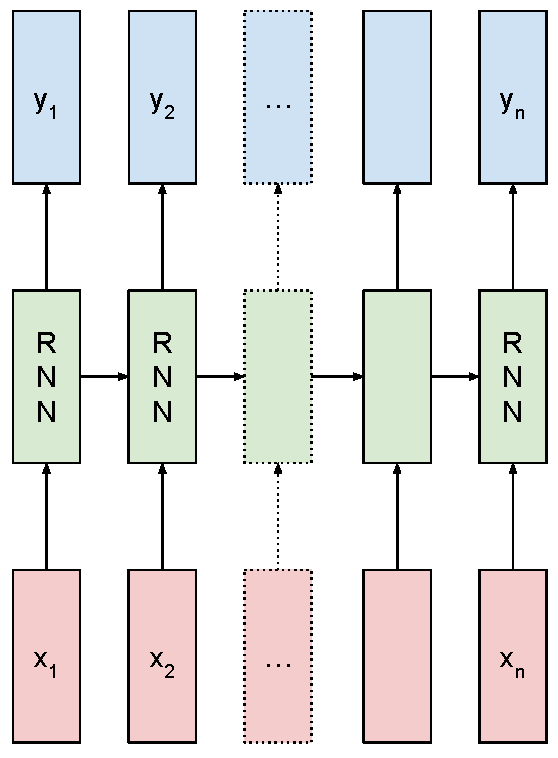
\includegraphics[height=7cm]{variable_input_output.pdf}
			\end{figure}
		\end{column}

		\begin{column}{.48\textwidth}
			\pause
			\vspace{1cm}
			How to solve the issue of varying input/output lengths?
			\pause
	
			\begin{enumerate}
				\item We \textbf{don't have to} stop generating after the last input
				\item We can only consider outputs up to a special \textbf{"end token"} 
			\end{enumerate}
			\pause
			Both of these approaches are not ideal
		\end{column}
\end{columns}
\end{frame}

\begin{frame}{Sequence-to-sequence models}

\begin{columns}[T] % align columns
	\begin{column}{.59\textwidth}
	
		\begin{figure}[h]
		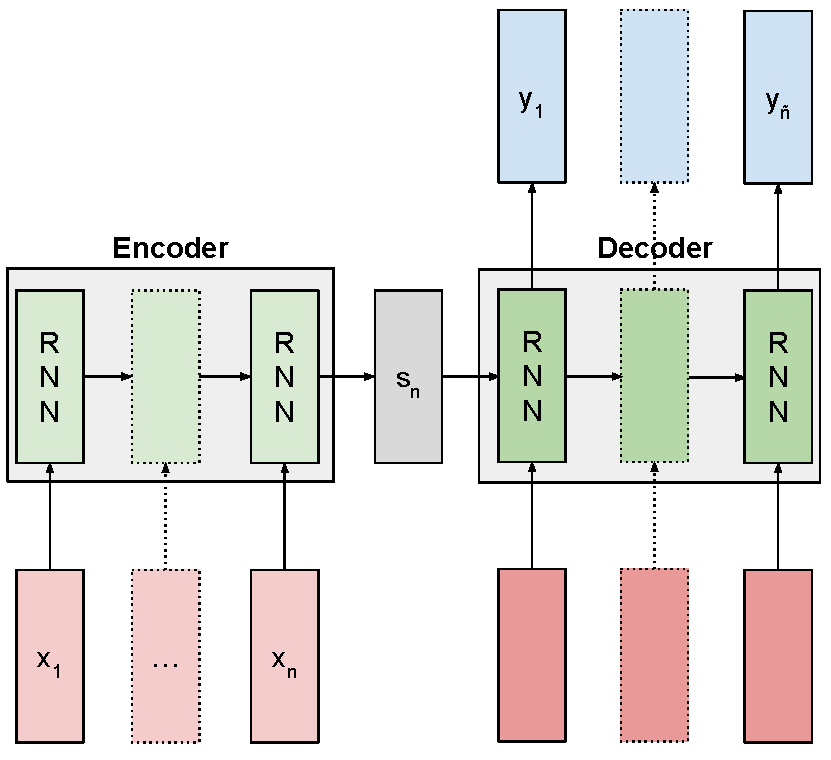
\includegraphics[height=7cm]{sequence_to_sequence_boxed.pdf}
	\end{figure}
	
	\end{column}
	\pause
	\begin{column}{.39\textwidth}
		\vspace{1cm}
		\textbf{Idea}: separate the solution into two networks
		\begin{itemize}
			\item \textbf{Encoder} (reader) RNN
			\item \textbf{Decoder} (writer) RNN
		\end{itemize}
		\pause
		Note:
		\begin{itemize}
			\item Encoder and decoder have \textbf{separate} parameters
			\item Initial state of decoder = \textbf{last state} of encoder
		\end{itemize}
	\end{column}
\end{columns}
\end{frame}
	
	

\begin{frame}[fragile]{The encoder-decoder architecture specifics}

\begin{enumerate}
\item How to \textbf{initialize} decoder hidden \textbf{state}?
\pause
\begin{itemize}
	\item $h_{0}^{dec} = h_{n}^{enc}$: simply copy the last encoder state
	\item $h_{0}^{dec} = \text{NN}_{\theta}(h_{n}^{enc})$: transform the last encoder state (\textbf{Why?})
\end{itemize}
\pause
\item When do we \textbf{stop generating} with the decoder?
\pause
\begin{itemize}
	\item We use a \textbf{special token} (\verb|<EOS>|, \verb|\n|) to indicate the end-of-sequence
	\item When the \textbf{maximum generation length} is exceeded
\end{itemize}
\pause
\item What are the \textbf{inputs} of the decoder?
\pause
\begin{itemize}
	\item The \textbf{previous output} of the decoder
	\begin{itemize}
		\item Teacher forcing (with probability $p$): use the \textbf{correct output} 
	\end{itemize}
	\pause
	\item What is the \textbf{initial input} $x^{dec}_0$?
	\pause
	\begin{itemize}
		\item A beginning-of-sequence \textbf{special token} (\verb|<BOS>|)
	\end{itemize}
\end{itemize}

\end{enumerate}

\end{frame}

\begin{frame}{The encoder-decoder architecture}

	\begin{columns}[T] % align columns
		\begin{column}{.59\textwidth}
		
			\begin{figure}[h]
			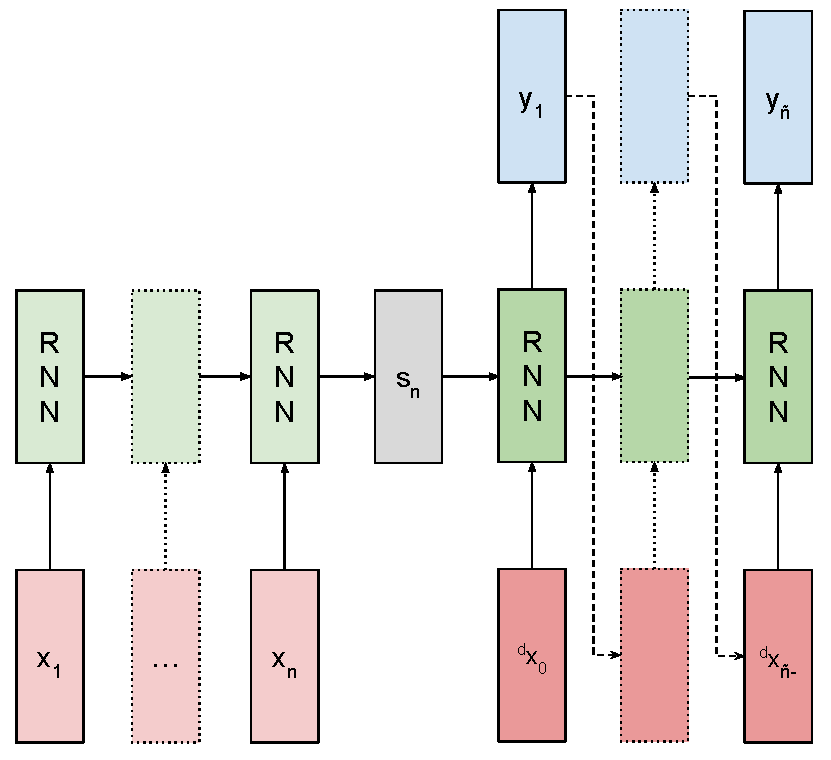
\includegraphics[height=7cm]{sequence_to_sequence_anno.pdf}
		\end{figure}
		
		\end{column}
		\pause
		\begin{column}{.39\textwidth}
			\vspace{2cm}
			Decoder inputs
			\begin{itemize}
				\item $x_0^{dec} = \text{<BOS>}$
				\item $x_i^{dec} = y_{i}^{dec}$ \textbf{if} no teacher forcing
				\item $x_i^{dec} = \hat{y}_{i}$ \textbf{if} we use teacher forcing 
			\end{itemize}
		\end{column}
	\end{columns}

\end{frame}

%\subsection{Text generation: beam search}

%\begin{frame}{Beam search decoding}
%	why: probability of sequence is low
%	greedy approach might not be best approach
%	todo
%\end{frame}

\begin{frame}[fragile]{Summary}

	\begin{itemize}
		\item Sequence generation tasks difficult to solve with a single RNN
		\item Encoder-decoder architecture: use two separate RNN networks
		\begin{itemize}
			\item The encoder reads the input text and compresses it into a fixed size vector
			\item The decoder uses the input text representation and generates output text
		\end{itemize}
		\item Encoder-decoder specifics:
		\begin{itemize}
			\item Special tokens: \verb|<BOS>|, \verb|<EOS>|
			\item Helping the network: teacher forcing
		\end{itemize}
	\end{itemize}

\end{frame}

\section{Overview of NLP tasks}

\begin{frame}{Overview of NLP tasks}

	\begin{figure}
		\centering
		\begin{subfigure}[b]{0.28\textwidth}
			\centering
			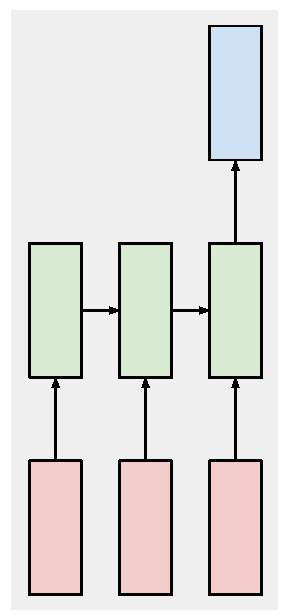
\includegraphics[height=5.5cm]{sequence_classification.pdf}
			\caption{Seq. classification}
			\label{fig:seqclf}
		\end{subfigure}
		\hfill
		\begin{subfigure}[b]{0.28\textwidth}
			\centering
			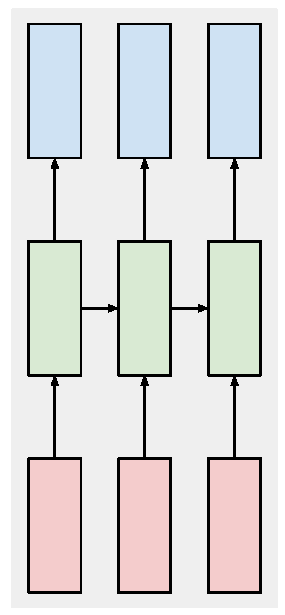
\includegraphics[height=5.5cm]{sequence_labeling.pdf}
			\caption{Seq. labeling}
			\label{fig:seqlab}
		\end{subfigure}
		\hfill
		\begin{subfigure}[b]{0.4\textwidth}
			\centering
			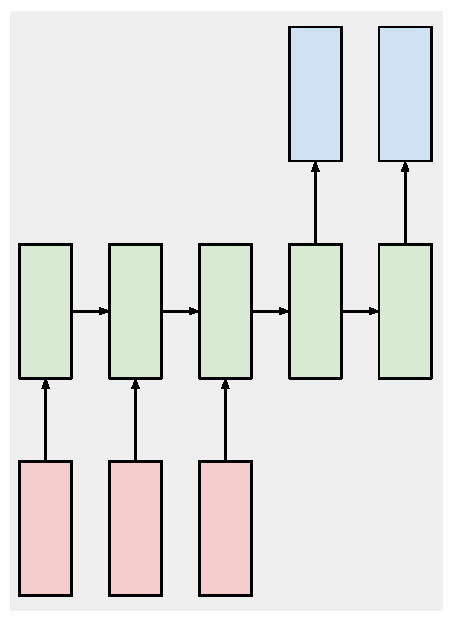
\includegraphics[height=5.5cm]{seq2seq.pdf}
			\caption{Sequence-to-sequence}
			\label{fig:seq2seq}
		\end{subfigure}
		   %\caption{}
		   %\label{fig:three graphs}
   \end{figure}
   
\end{frame}

\begin{frame}{Sequence classification}
	\begin{columns}[T] % align columns
		\begin{column}{.49\textwidth}
		
			\begin{figure}[h]
			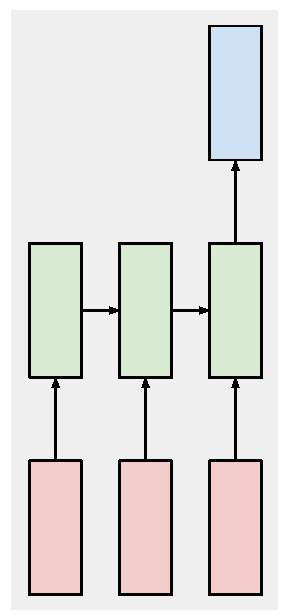
\includegraphics[height=6cm]{sequence_classification.pdf}
		\end{figure}
		
		\end{column}
		\begin{column}{.49\textwidth}
			\vspace{1cm}
			Determine a label for one (or more) text sequences
			\begin{itemize}
				\item News article categorization, sentiment analysis,... 
			\end{itemize}
			\pause
			\textbf{Approach}
			\begin{enumerate}
				\item Encode sequence(s) into a sequence representation
				\item Pass sequence representation to decoder layer
			\end{enumerate}
		\end{column}
	\end{columns}

\end{frame}

\begin{frame}{Sequence labeling}
	\begin{columns}[T] % align columns
		\begin{column}{.49\textwidth}
		
			\begin{figure}[h]
				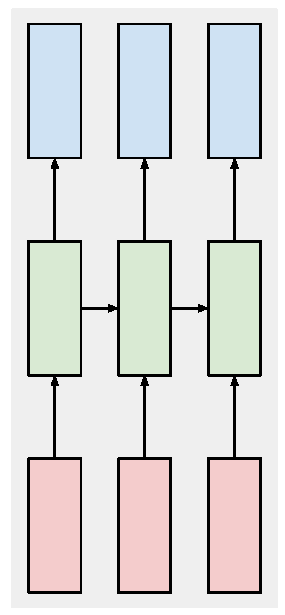
\includegraphics[height=6cm]{sequence_labeling.pdf}
			\end{figure}
		
		\end{column}
		\begin{column}{.49\textwidth}
			\vspace{1cm}
			Determine a label for \textbf{each element} of a sequence
			\begin{itemize}
				\item Part-of-speech tagging, named entity recognition,...
			\end{itemize}
			\pause
			\textbf{Approach}
			\begin{enumerate}
				\item Encode (contextualize) sequence elements
				\item Pass representation of each element to (same) decoder layer
			\end{enumerate}
		\end{column}
	\end{columns}

\end{frame}

\begin{frame}{Sequence to sequence}
	\begin{columns}[T] % align columns
		\begin{column}{.49\textwidth}
		
			\begin{figure}[h]
			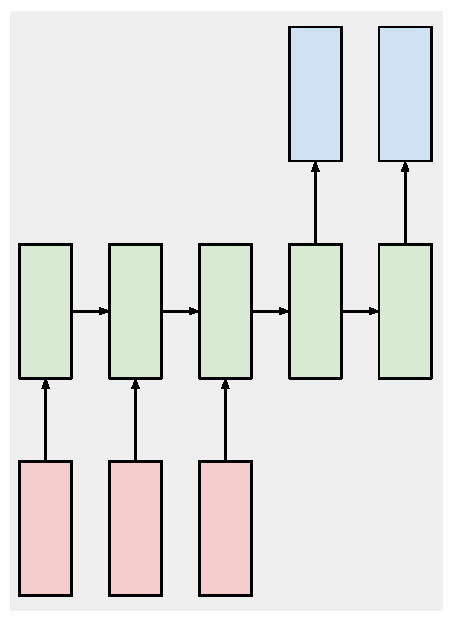
\includegraphics[height=6cm]{seq2seq.pdf}
		\end{figure}
		
		\end{column}
		\begin{column}{.49\textwidth}
			\vspace{1cm}
			Generate a sequence of tokens given a sequence of tokens
			\begin{itemize}
				\item Machine translation, summarization, text generation,...
			\end{itemize}
			\textbf{Approach}
			\begin{enumerate}
				\item Use encoder network to encode input sequence
				\item Use decoder network to generate output sequence
			\end{enumerate}
		\end{column}
	\end{columns}

\end{frame}

\section{The attention mechanism}

\begin{frame}{Motivation}
... we apply our multilayer bidirectional LSTM network to a machine translation problem.

What \textbf{types of instances} would it perform bad on? \textbf{Why}?

\vspace{1em}
\pause
The problem of \textbf{long dependencies}
\begin{itemize}
		\item The hidden state of a RNN network is \textbf{finite}
		\item The more tokens the RNN reads, the less it remembers \textbf{individual} tokens
	\end{itemize}

\end{frame}


\begin{frame}{The long dependency problem}
	\begin{figure}[h]
		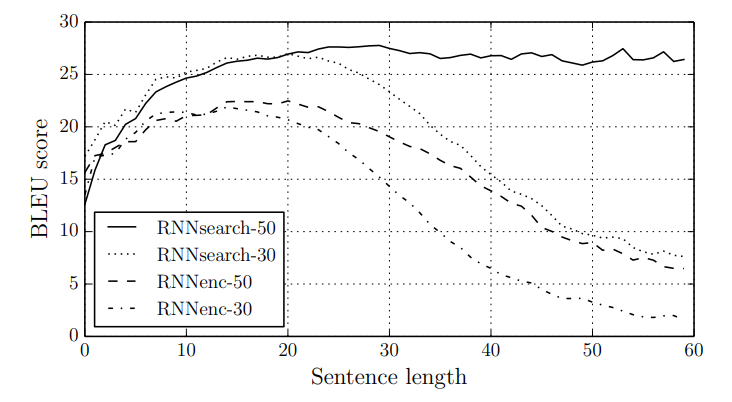
\includegraphics[height=6cm]{sequence_length}
		\caption*{Figure from \cite{bahdanau2014neural}}
	\end{figure}	
\end{frame}
	

\begin{frame}{The attention mechanism: intuition}

\hspace*{\parindent}	\emph{``When I’m translating a sentence, I pay special attention to the word I’m presently translating.
	When I’m transcribing an audio recording, I listen carefully to the segment I’m actively writing down. 
	And if you ask me to describe the room I’m sitting in, I’ll glance around at the objects I’m describing as I do so.''}

-- By \href{https://distill.pub/2016/augmented-rnns/}{\underline{Christopher Olah}}

\pause
\vspace{1em}
\textbf{Idea}: our recurrent state does not have perfect memory of previous content.
However, it should know which content \textbf{was relevant}.
\begin{itemize}
	\item Attention allows the network to \textbf{view previous states}
\end{itemize} 

\end{frame}

\begin{frame}{The attention mechanism: visual context}
	\begin{figure}[h]
		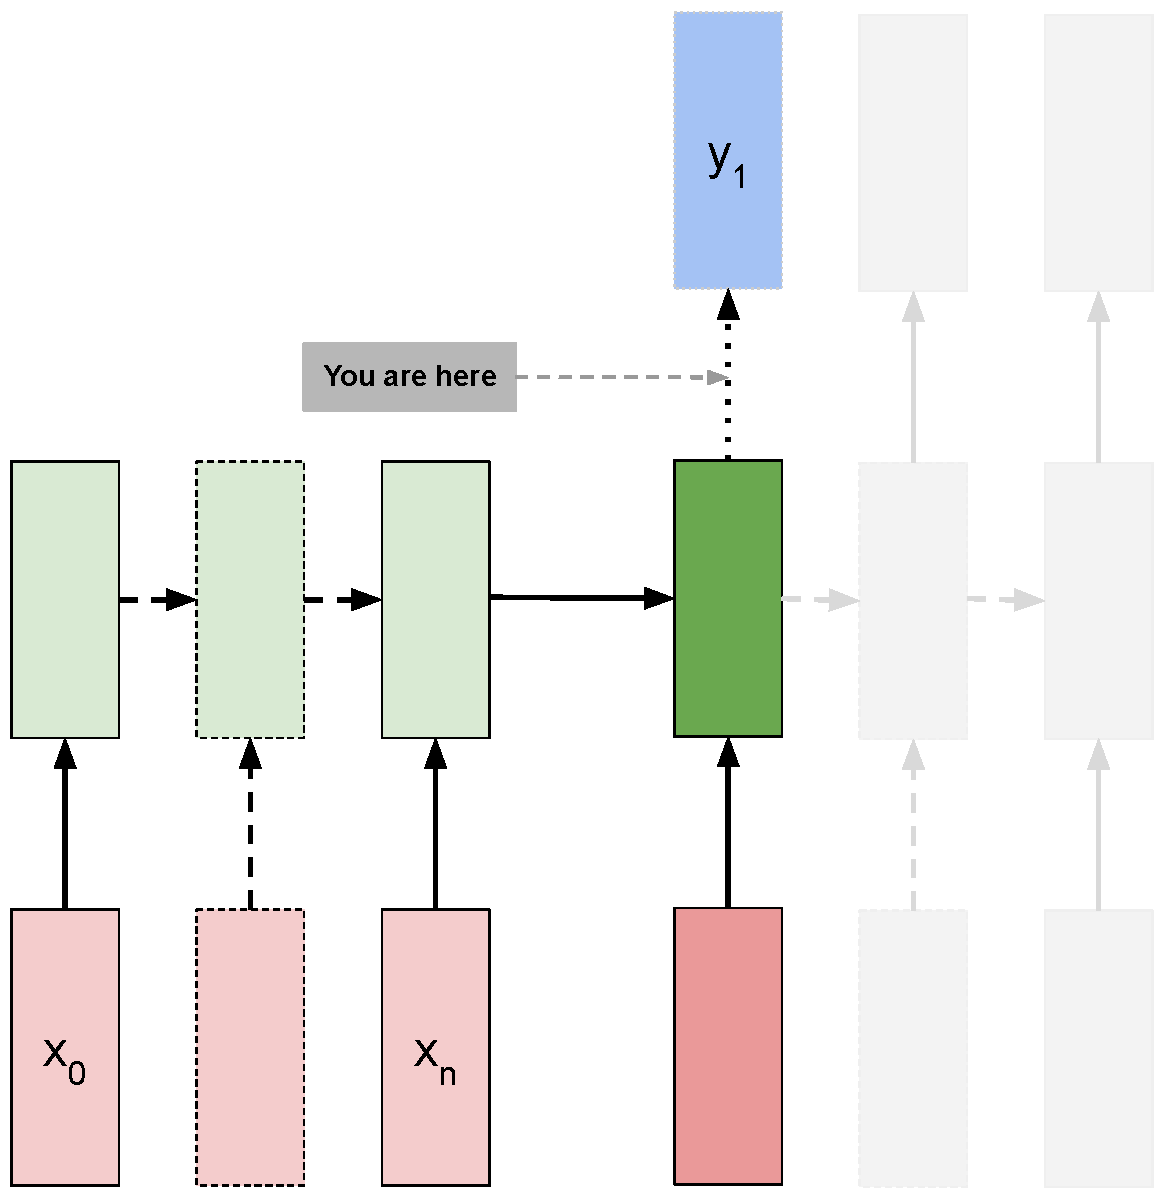
\includegraphics[height=7cm]{seq2seq_attention_motivation.pdf}
	\end{figure}	
\end{frame}

\begin{frame}{The attention mechanism: formalization}

A standard encoder-decoder network produces a \textbf{sequence of states} $s_{i}^{\text{enc/dec}}$
\pause

At a (decoder) time-step $t$, we want to obtain a \textbf{fixed size} update (with respect to sequence length $N$) representing \textbf{relevant information} from the past
\pause

\vspace{1em}
We \textbf{have}: $s^{\text{dec}}_t$, $S^{\text{enc}} = \{s_i^{\text{enc}}\}_{i=1}^n$, we \textbf{want}: $a \approx \text{relevant}(S^{\text{enc}}|s^{\text{dec}}_t)$

\pause
\vspace{1em}
\begin{enumerate}
	\item Compute the \textbf{energy} (similarity, relevance) function between two dense vectors (the \textbf{current} decoder state and \textbf{one} encoder state)
	$$
		\alpha_i = \text{attn}(s_i^{\text{enc}}, s_t^{\text{dec}}) \pause \approx \underbrace{s_i^{\text{enc}} \cdot s_t^{\text{dec}}}_{\text{dot product}}
	$$
	\seti
\end{enumerate}

\end{frame}

\begin{frame}{The attention mechanism: formalization}
	
	\begin{enumerate}
		\conti
		\item We \textbf{scale} the output of the dot product to preserve scale of variance (\cite{Vaswani.et.al.2017}) (otherwise values get too large -- issue for next step)
			$$
				\hat{\alpha}_i = \frac{s_i^{\text{enc}} \cdot s_t^{\text{dec}}}{\sqrt{d_{\text{dec} } } }
			$$
			\pause
			$d_{\text{dec}}$ is the dimensionality of the decoder state (Why decoder?)
			\pause
		\item We \textbf{normalize} the energy to a probability distribution over (encoder) states
		$$
			\alpha_i = \text{softmax}(\hat{\alpha}_i) = \frac{e^{\hat{\alpha_i}}}{\sum_j^N e^{\hat{\alpha}_j}}
		$$
		\seti
		\pause
		Why would the scale of $\hat{\alpha}_i$ be an issue? \pause (softmax)

	\end{enumerate}

\end{frame}

\begin{frame}{The attention mechanism: formalization}
	We now have \textbf{importance} $\alpha_i$ of each (encoder) element. How to produce the \textit{summary} $a$?

	\begin{enumerate}
		\conti
		\item We can \textbf{sum} over the elements with $\alpha_i$ as the elements' weight!
		$$
			a = \sum_i^n \alpha_i s_i^{\text{enc}}
		$$

	\end{enumerate}

\pause

\begin{itemize}
	\item $\alpha_i \approx $ \textbf{importance} of state $s_i^{\text{enc}}$   
	\item $s_i^{\text{enc}} \approx $ information we are \textbf{recalling} 
\end{itemize}

\pause

This is the initial formulation of \textbf{dot-product} \textbf{encoder-decoder} attention.
\pause
\begin{itemize}
	\item Attention is a weighted (convex) sum over a set of elements.
\end{itemize}
	
\end{frame}


\begin{frame}{The attention mechanism: visual context}

	\begin{columns}[T]
		\begin{column}{0.49\textwidth}
			\begin{figure}[h]
				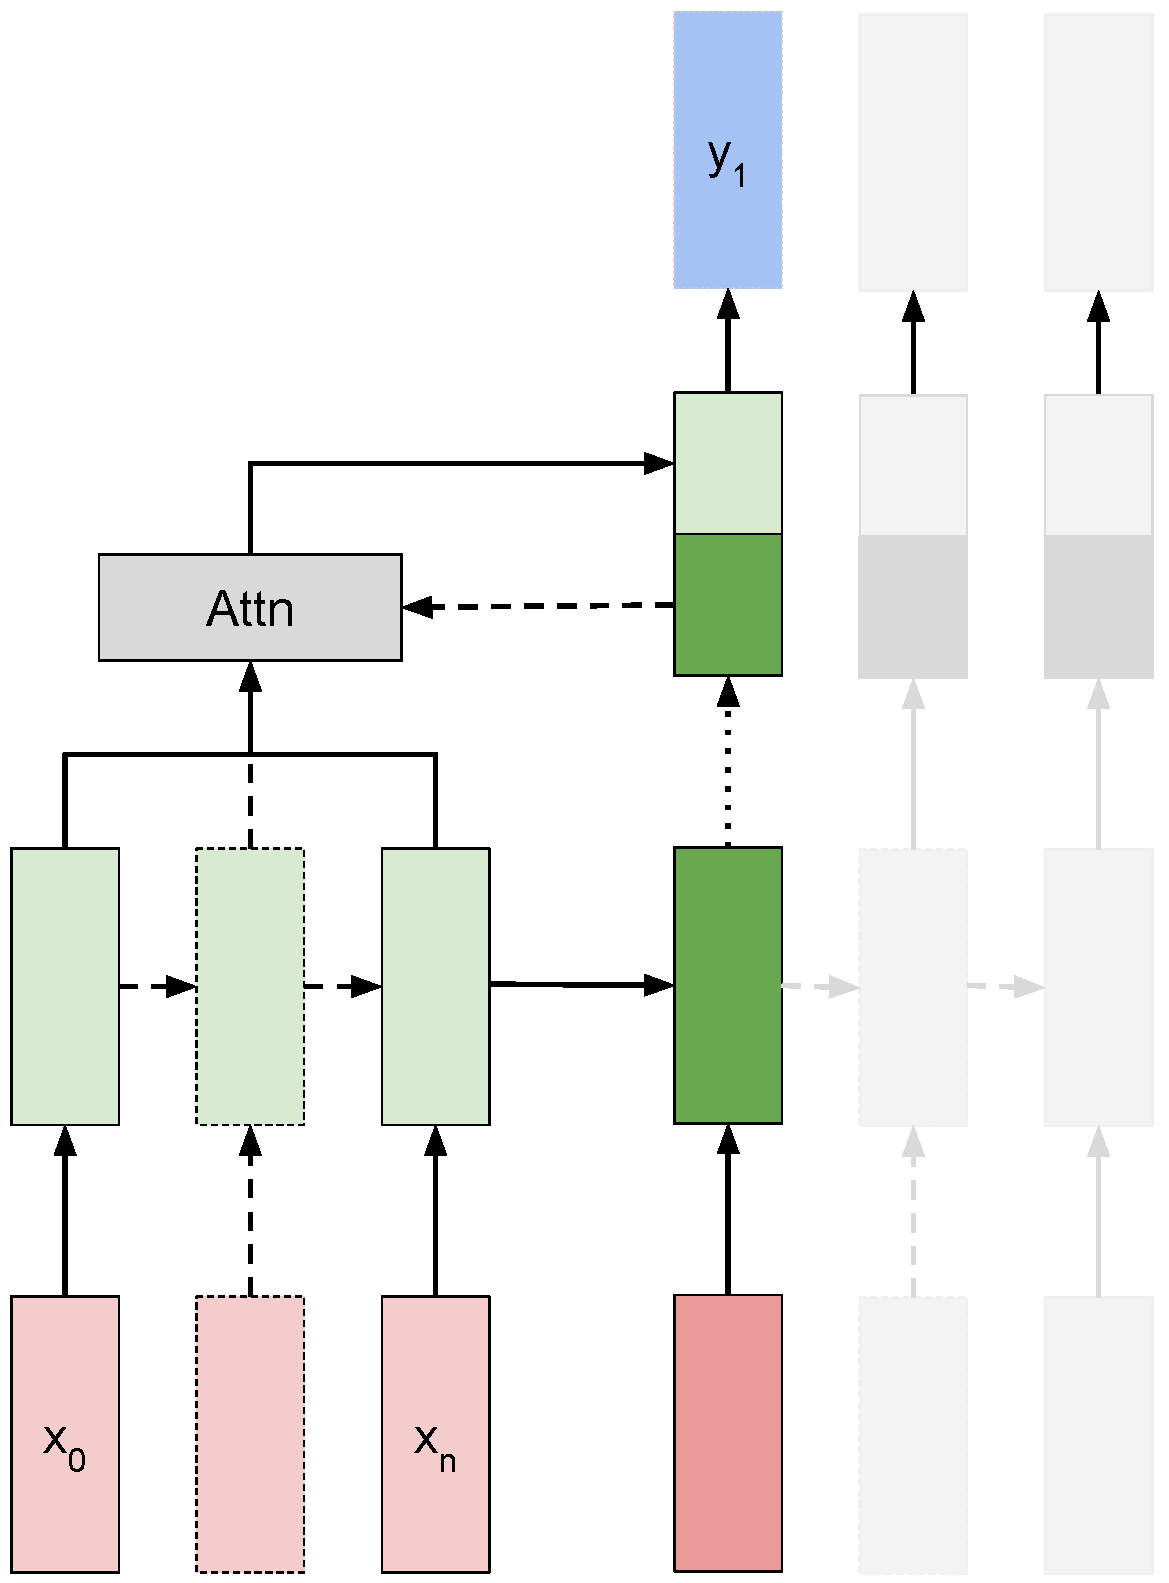
\includegraphics[height=6.5cm]{seq2seq_attention_t1.pdf}
			\end{figure}	
		\end{column}
		\begin{column}{0.49\textwidth}
			\begin{enumerate}
			\pause
			\item Given the current decoder state $s^{\text{dec}}_t$ and encoder states $S^{\text{enc}} = \{s_i^{\text{enc}}\}_{i=1}^n$, 
				compute the output of the attention mechanism $a_t = \sum_i^n \alpha_i s_i^{\text{enc}}$
			\pause
			\item \textbf{Concatenate} the output of attention and the current decoder state $\hat{s}_t^{\text{dec}} = [s^{\text{dec}}_t | a_t]$
			\pause
			\item Predict the next token $y_t$
			\end{enumerate}
			\end{column}
	\end{columns}
	
\end{frame}

\begin{frame}{The attention mechanism: visalizing attention}
	\begin{figure}[h]
		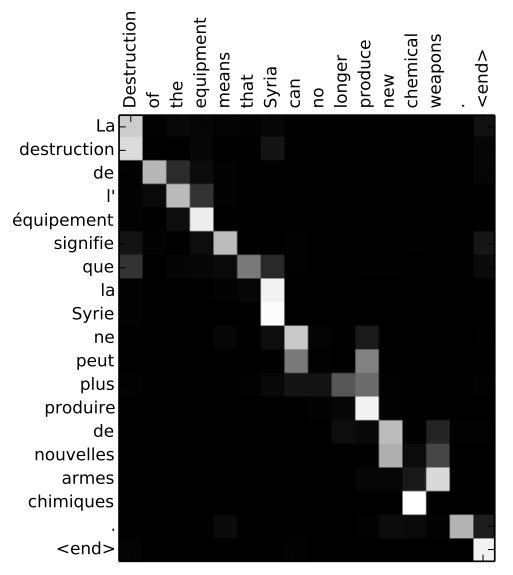
\includegraphics[height=6cm]{translation_heatmap}
		\caption*{White = attention (btw enc. and dec. state) is high. Black = attention is low.\\ Figure from \cite{bahdanau2014neural}.}
	\end{figure}	
\end{frame}

\begin{frame}{The attention mechanism: effect of attention}
	\begin{figure}[h]
		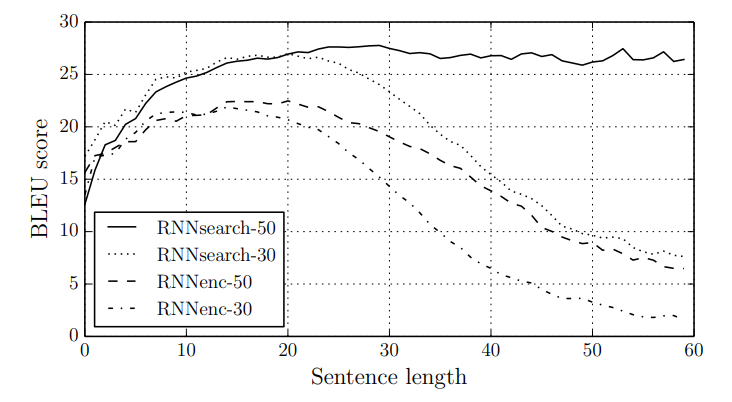
\includegraphics[height=6cm]{sequence_length}
		\caption*{RNNsearch architectures use attention. Figure from \cite{bahdanau2014neural}.}
	\end{figure}	
\end{frame}


\subsection{Abstracted attention mechanism}


\begin{frame}{The attention mechanism: abstraction}
	Components of the attention mechanism
	\begin{enumerate}
		\item The \textbf{query} $q = f_q(s^{\text{dec}}_t); \quad q \in \mathbb{R}^{d_q}$
		\begin{itemize}
			\item The query is the state representation based on which we \textbf{seek information}
		\end{itemize}
		\pause

		\item The \textbf{keys} $K = f_k(\{s^{\text{enc}}_i\}_{i=1}^n); \quad K \in \mathbb{R}^{n \times d_k}$
		\begin{itemize}
			\item The keys are the representations we \textbf{compare} the query to
		\end{itemize}
		\pause

		\item The \textbf{values} $V = f_v(\{s^{\text{enc}}_i\}_{i=1}^n); \quad V \in \mathbb{R}^{n \times d_v}$
		\begin{itemize}
			\item The values are the representations we \textbf{sum over} given the attention scores 
		\end{itemize}
	\end{enumerate} 
	\pause
	Where $f_q, f_k, f_v$ are arbitrary functions (neural network layers).

	\pause
	\noindent\begin{minipage}{0.4\textwidth}
				\begin{equation}
					a = \sum_i^n \alpha_i v_i
				\end{equation} 
		\end{minipage}%
		\begin{minipage}{0.2\textwidth}
		\end{minipage}
		\begin{minipage}{0.4\textwidth}
			\begin{equation}
				\hat{\alpha}_i = \frac{q^T \cdot k_i}{\sqrt{d_{\text{dec} } } }
			\end{equation}
		\end{minipage}\vskip1em
	
\end{frame}

\subsection{The attention mechanism: design choices}

\begin{frame}{The attention mechanism: choices}
	Key choices when using the attention mechanism:
	\begin{enumerate}
		\item The \textbf{energy} (similarity, relevance) function
		\begin{itemize}
			\item Defines how we \textbf{compute energy} between two state representations
		\end{itemize}

		\item Parametrization
		
		\begin{itemize}
			\item Determines how (and if) we \textbf{apply transformations} to attention components
		\end{itemize}
		
		\item Direction
		
		\begin{itemize}
			\item Determines which components we \textbf{attend over}
		\end{itemize}

	\end{enumerate}
\end{frame}

\begin{frame}{The attention mechanism: energy}
	\begin{enumerate}
		\item \underline{The \textbf{energy} (similarity, relevance) function}
		\pause
		\begin{itemize}
			\item Dot product attention
				$$
					\hat{\alpha}_i = \frac{q^T \cdot k_i}{\sqrt{d_k} }
				$$
			\pause
			\begin{itemize}
				\item Requires $\text{dim}(q) = \text{dim}(k)$
				\item Introduces \textbf{no additional parameters}
			\end{itemize}

		\end{itemize}
	\end{enumerate}
\end{frame}


\begin{frame}{The attention mechanism: energy}
	\begin{enumerate}
		\item \underline{The \textbf{energy} (similarity, relevance) function}
		
		\begin{itemize}
			\item Bahdanau (\textbf{tanh}) attention ($[\cdot|\cdot]$ = concatenate)
				$$
					\hat{\alpha}_i = W_2 \text{tanh}(W_1 [q|k_i])
				$$
			\pause
			\begin{itemize}
				\item \textbf{No requirements} on dimensions of inputs (states)
				\item Additional parameters $W_1 \in \mathbb{R}^{(d_{q}+d_{k})\times h}$, $W_2 \in \mathbb{R}^{h}$
				\item $h$ is the dimension of the \textbf{attention hidden layer}
			\end{itemize}
		\end{itemize}
	\end{enumerate}
\end{frame}


\begin{frame}{The attention mechanism: energy}
	\begin{enumerate}
		\item \underline{The \textbf{energy} (similarity, relevance) function}
		\begin{itemize}
			\item \textbf{Bilinear} attention
			$$
				\alpha_i =q^T W k_i
			$$
			\pause
			\begin{itemize}
				\item \textbf{No requirements} on dimensions of states
				\item Additional parameters $W \in \mathbb{R}^{d_{q} \times d_{k}}$
			\end{itemize}
		\end{itemize}
		\seti
	\end{enumerate}
\end{frame}

\begin{frame}{The attention mechanism: parametrization}
	\begin{enumerate}
		\conti
		\item \underline{Parametrizations of inputs \& outputs}

		Remember: $f_q, f_k, f_v$ are arbitrary functions (neural network layers).
		\pause
		
		\hspace{1em} What are the most common ways to parametrize these functions?

		\pause
		\begin{itemize}
			\item Linear transformations: $f_{\{q,k,v\}} \in \mathbb{R}^{d_{\{q,k,v\}\_in} \times d_{\{q,k,v\}}}$
		\end{itemize}
		\pause
		\vspace{1em}

		\textbf{Intuition}: hidden states contain information which is not relevant for \textbf{computing energy} (query, keys) or \textbf{retrieving information} (values) -- linear transformations can filter (map to null space) unnecessary information.
		\seti
	\end{enumerate}

\end{frame}

\begin{frame}{The attention mechanism: direction}

	\begin{columns}[T] % align columns
		\begin{column}{.48\textwidth}
			\begin{figure}[h]
				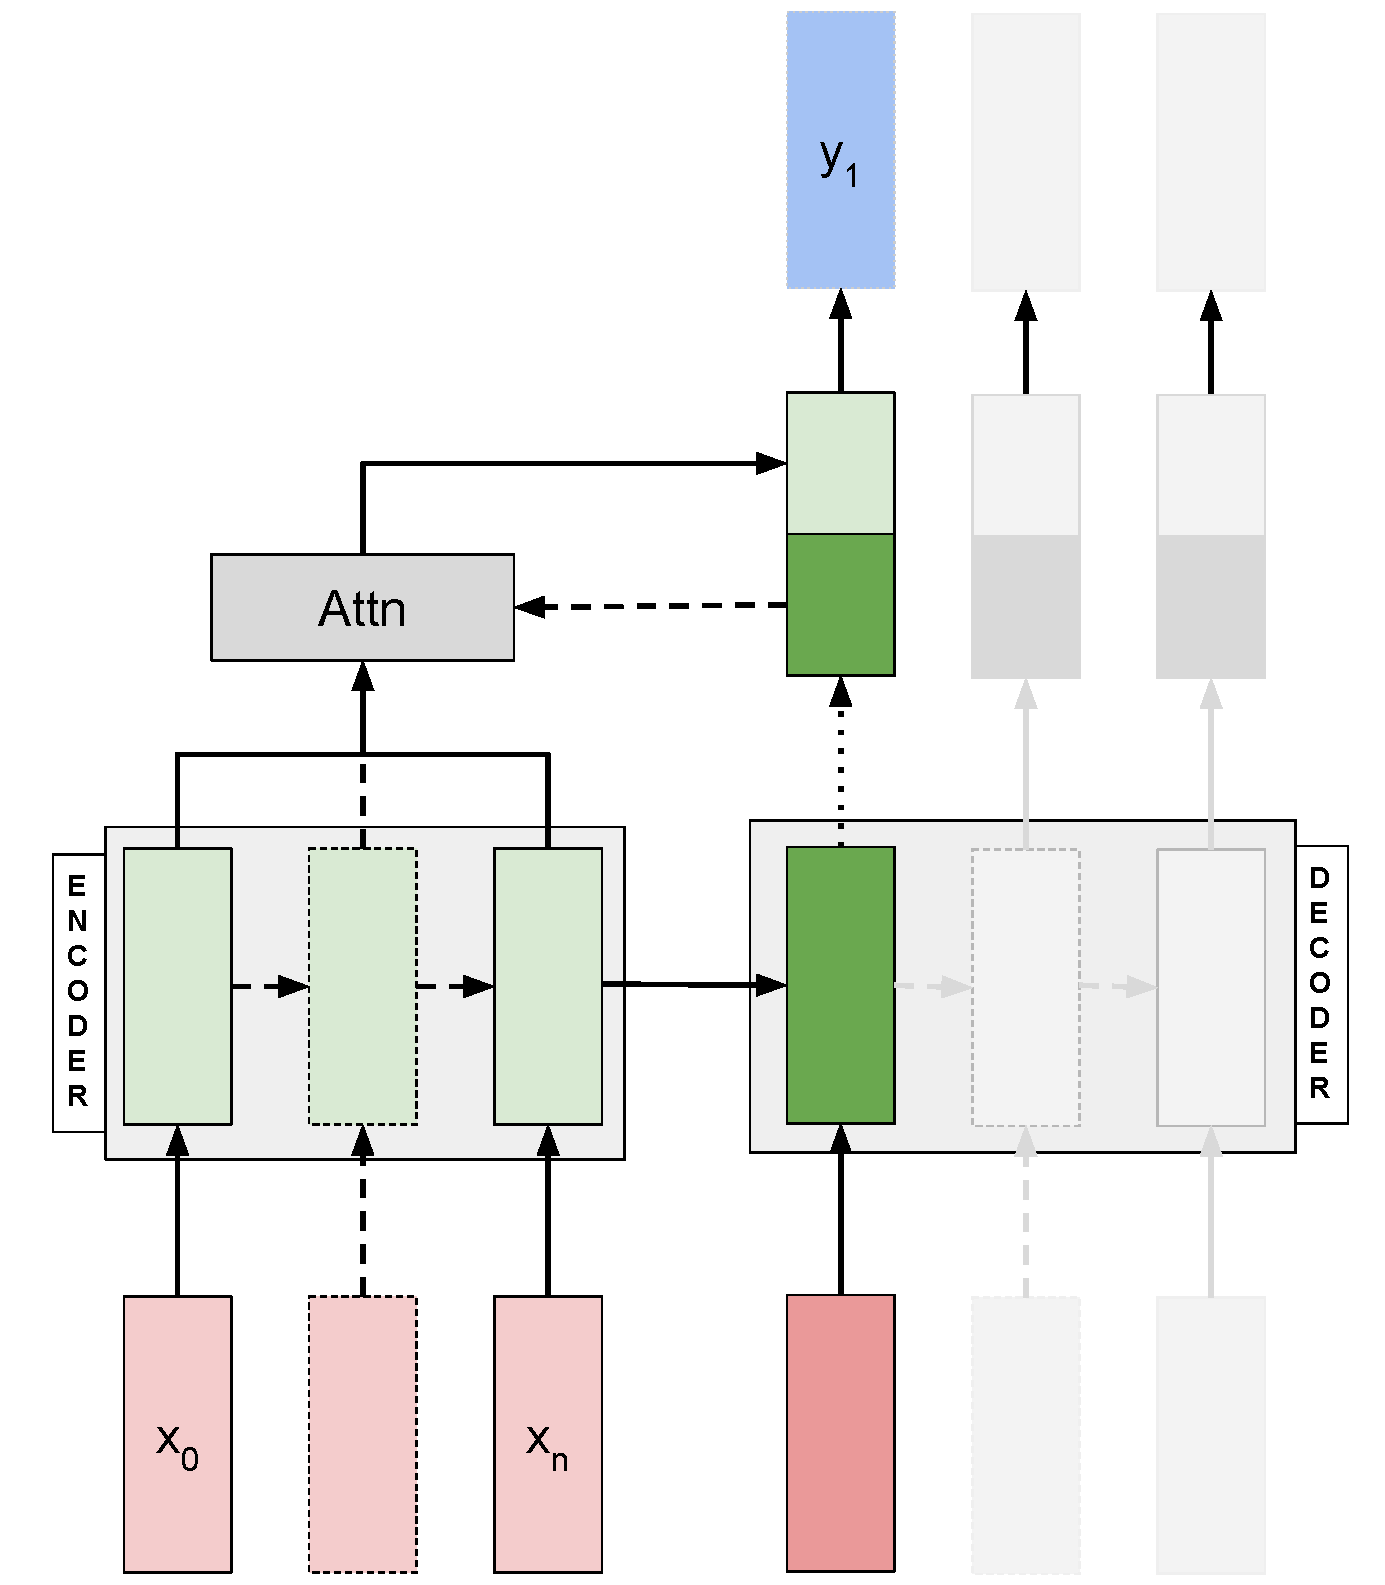
\includegraphics[height=7cm]{seq2seq_attn_encdec.pdf}
			\end{figure}
		\end{column}
		\begin{column}{.48\textwidth}
			\begin{enumerate}
				\conti
				\item \underline{Direction of attention}
		
				We have so far only shown encoder-decoder \textbf{cross attention}
				\pause
				\hspace{1em}
				
				Flavors of attention
				\begin{itemize}
					\item \textbf{Cross-attention}:
					between encoder and decoder (or any \textbf{query} and \textbf{a sequence} of hidden states)
				\end{itemize}
			\end{enumerate}
		\end{column}
	\end{columns}

\end{frame}


\begin{frame}{The attention mechanism: direction}

	\begin{columns}[T] % align columns
		\begin{column}{.48\textwidth}
			\begin{figure}[h]
				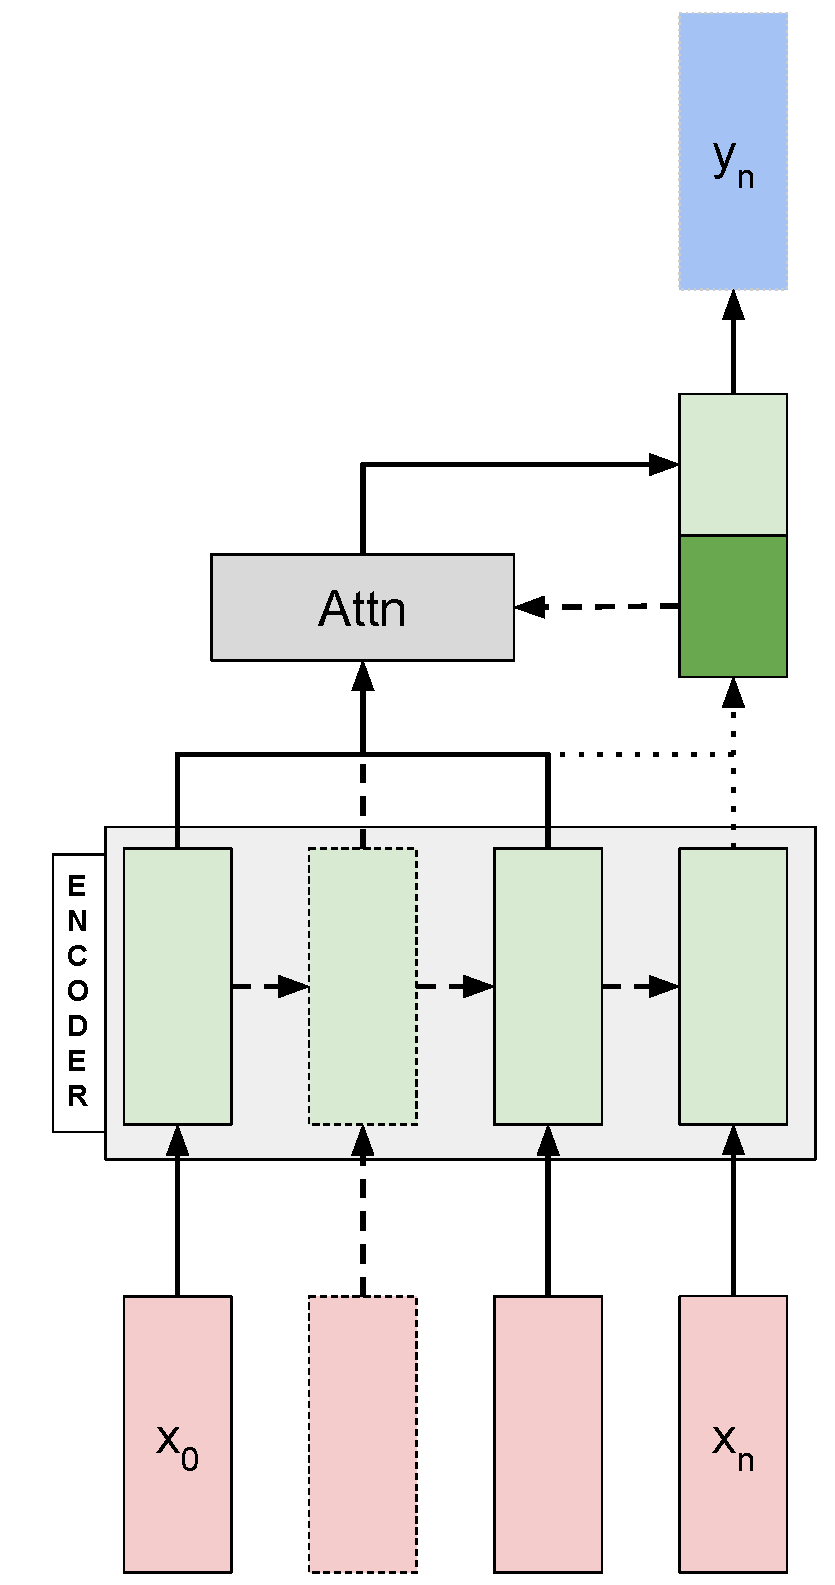
\includegraphics[height=7cm]{seq2seq_selfattn.pdf}
			\end{figure}
		\end{column}
		\begin{column}{.48\textwidth}
			\begin{enumerate}
				\conti
				\item \underline{Direction of attention}
		
				\textcolor{gray}{We have so far only shown encoder-decoder \textbf{cross attention}}
				\hspace{1em}
				
				Flavors of attention
				\begin{itemize}
					\item \textbf{Self-attention}:
					between a sequence of hidden states and a query originating from the \textbf{same sequence} of hidden states
				\end{itemize}
			\end{enumerate}
		\end{column}
	\end{columns}


\end{frame}

\section*{Recap}

% **Content**
%
%* Vanilla RNNs (and maybe vanishing/exploding gradient?)
%* LSTM cells
%* Bi-Directional LSTMs
%* Domain adaptation and multi-task learning (?) 
%
%**Notes**
%
%efficiency, bidirectionality, multi-layer RNNs, how to apply to different tasks, how to ensure no data leakage
%connection to LMs (using RNNs)?
%
%* Domain adaptation and multi-task learning (?) - should be somewhere early too

\begin{frame}{Take aways}
	
\begin{itemize}
	\item Encoder-decoder architecture -- used for generating variable (wrt. input) length sequences
	\item Three classes of sequence problems: classification, labeling \& seq2seq
	\item RNNs are bad at long dependencies
	\item Attention mechanism allows networks to \textit{look at} previous states
	\item Abstraction of attention mechanism: (1) query, (2) keys, (3) values
	\item Design choices of attention: (1) energy function, (2) parametrization, (3) direction
\end{itemize}
	
\end{frame}



\begin{frame}{License and credits}

	\begin{columns}
		\begin{column}{0.7\textwidth}
			Licensed under Creative Commons Attribution-ShareAlike 4.0 International (CC BY-SA 4.0)
		\end{column}
		\begin{column}{0.2\textwidth}
			
\includegraphics[width=0.9\linewidth]{img/cc-by-sa-icon.pdf}
		\end{column}
	\end{columns}
	
	\bigskip
	
	Credits
	
	\begin{scriptsize}
		
		Martin Tutek
		
		Content from ACL Anthology papers licensed under CC-BY \url{https://www.aclweb.org/anthology}
		
	
	\end{scriptsize}
	
\end{frame}



\end{document}

